\documentclass{article}
\usepackage{amsmath}  % Pacchetto per migliorare la resa matematica
\usepackage{amssymb}  % Per simboli matematici aggiuntivi
\usepackage{graphicx}
\usepackage[export]{adjustbox}
\usepackage{float}


\begin{document}

un obbd (Ordered binary decision-diagram) è una rappresentazione di una funzione booleana sotto forma di DAG radicato.

\begin{figure}[H]
    \centering
    \includegraphics[max width=\linewidth, max height=0.9\textheight, keepaspectratio]{Resources/TavolaVerità.png}
    \caption{Tavola di verità e albero di decisione di una funzione booleana, archi tratteggiati indicano il caso in cui la variabile sia 0, archi continui indicano il caso in cui la variabile sia 1}
    \label{fig:tavolaVerita}
\end{figure}

Nel caso particolare della figura 1 il grafo in esempio è anche un albero.
Ogni vertice non terminale $v$ è etichettato con una variabile $var(v)$ (un parametro della funzione) e ha due figli, $lo(v)$ (arco tratteggiato) che corrisponde al caso in cui il valore di $var(v)$ è $0$ e $hi(v)$ (arco continuo) che corrisponde al caso in cui il valore di $var(v)$ è $1$, i nodi terminali sono etichettati con $0$ o $1$.
Il valore della funzione, dato un assegnamento delle variabili, è dato dalla foglia del percorso radice-foglia ottenuto percorrendo gli archi secondo i valori assegnati alle variabili.
Inoltre le variabili sono ordinate in base a "quale appare prima", nell'esempio della figura 1 l'ordine è $x_1<x_2<x_3$.
Su un obdd si possono compiere 3 operazioni che non alterano la funzione da esso rappresentata:

\textbf{rimozione dei nodi duplicati terminali:} si eliminano tutti i nodi terminali tranne uno per ogni label e si indirizzano tutti gli archi entranti dei nodi eliminati verso quello rimasto con la stessa label (quindi si avranno due nodi terminali: $1$ e $0$)

\textbf{rimozione dei nodi duplicati interni:} se esistono due nodi interni $v$ e $u$ con $var(v) = var(u)$, $lo(v) = lo(u)$ e $hi(v) = hi(u)$ allora si elimina uno dei due e si indirizzano tutti i suoi archi entranti verso quello rimanente.

\textbf{rimozione dei test ridondanti:} se esiste un nodo $v$ con $lo(v) = hi(v)$ allora si elimina il nodo $v$ e si indirizzano tutti i suoi archi entranti verso $lo(v)$, (se i due archi uscenti di $v$ portano entrambi verso lo stesso nodo allora controllare il valore di $v$ è inutile)

\begin{figure}[H]
    \centering
    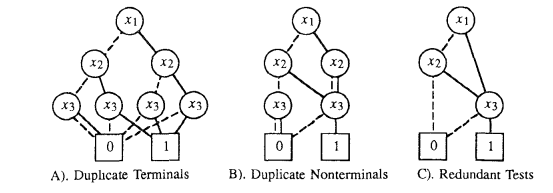
\includegraphics[max width=\linewidth, max height=0.9\textheight, keepaspectratio]{Resources/figure2obdd.png}
    \caption{riduzioni applicate all'albero della figura 1}
    \label{fig:riduzioni}
\end{figure}

Con $f\rvert_{x_i\leftarrow k}$ indichiamo una resitrizione della funzione $f$ in cui la variabile $x_i$ assume per forza valore $k \in \{0,1\}$, quindi su una funzione $f(x_1,x_2,x_3) \quad
f\rvert_{x_1\leftarrow 0} = f(0, x_2, x_3)$.
Inoltre indichiamo con $\cdot$ l'operazione AND, con $+$ l'operazione OR e con $\bar{x}$ la negazione di $x$
Ora possiamo riscrivere una funzione come: $f = (\bar{x} \cdot f\rvert_{x \leftarrow 0}) + (x \cdot f\rvert_{x \leftarrow 1})$, questa scrittura viene chiamata espansione di shannon.

Tramite l'operazione Apply è possibile creare una nuova funzione $f \langle op \rangle g$  dati come argomenti due funzioni $f$ e $g$(con lo stesso ordine di variabili) e un operatore booleano binario $\langle op \rangle$ (OR, AND, ...).
Possiamo sfruttare l'espansione di shannon per riscrivere la funzione: $f \langle op \rangle g = \bar{x} \cdot (f \langle op \rangle g \rvert_{x \leftarrow 0}) + x \cdot (f \langle op \rangle g \rvert_{x \leftarrow 1}) =  \bar{x} \cdot (f\rvert_{x \leftarrow 0} \langle op \rangle g\rvert_{x \leftarrow 0}) + x \cdot (f\rvert_{x \leftarrow 1} \langle op \rangle g \rvert_{x \leftarrow 1})$ 
Da notare che se $x$ è la variabile della radice $r$ di un grafo che rappresenta la funzione $f$ allora la funzione $f \rvert _{x \leftarrow 0 }$ è rappresentata dal sottografo radicato in $lo(r)$ analogamente $f \rvert _{x \leftarrow 1}$ è rappresentata dal sottografo radicato in $hi(r)$ quindi avendo due grafi che hanno la stessa variabile come radice possiamo unirli in questo modo

\begin{figure}[H]
    \centering
    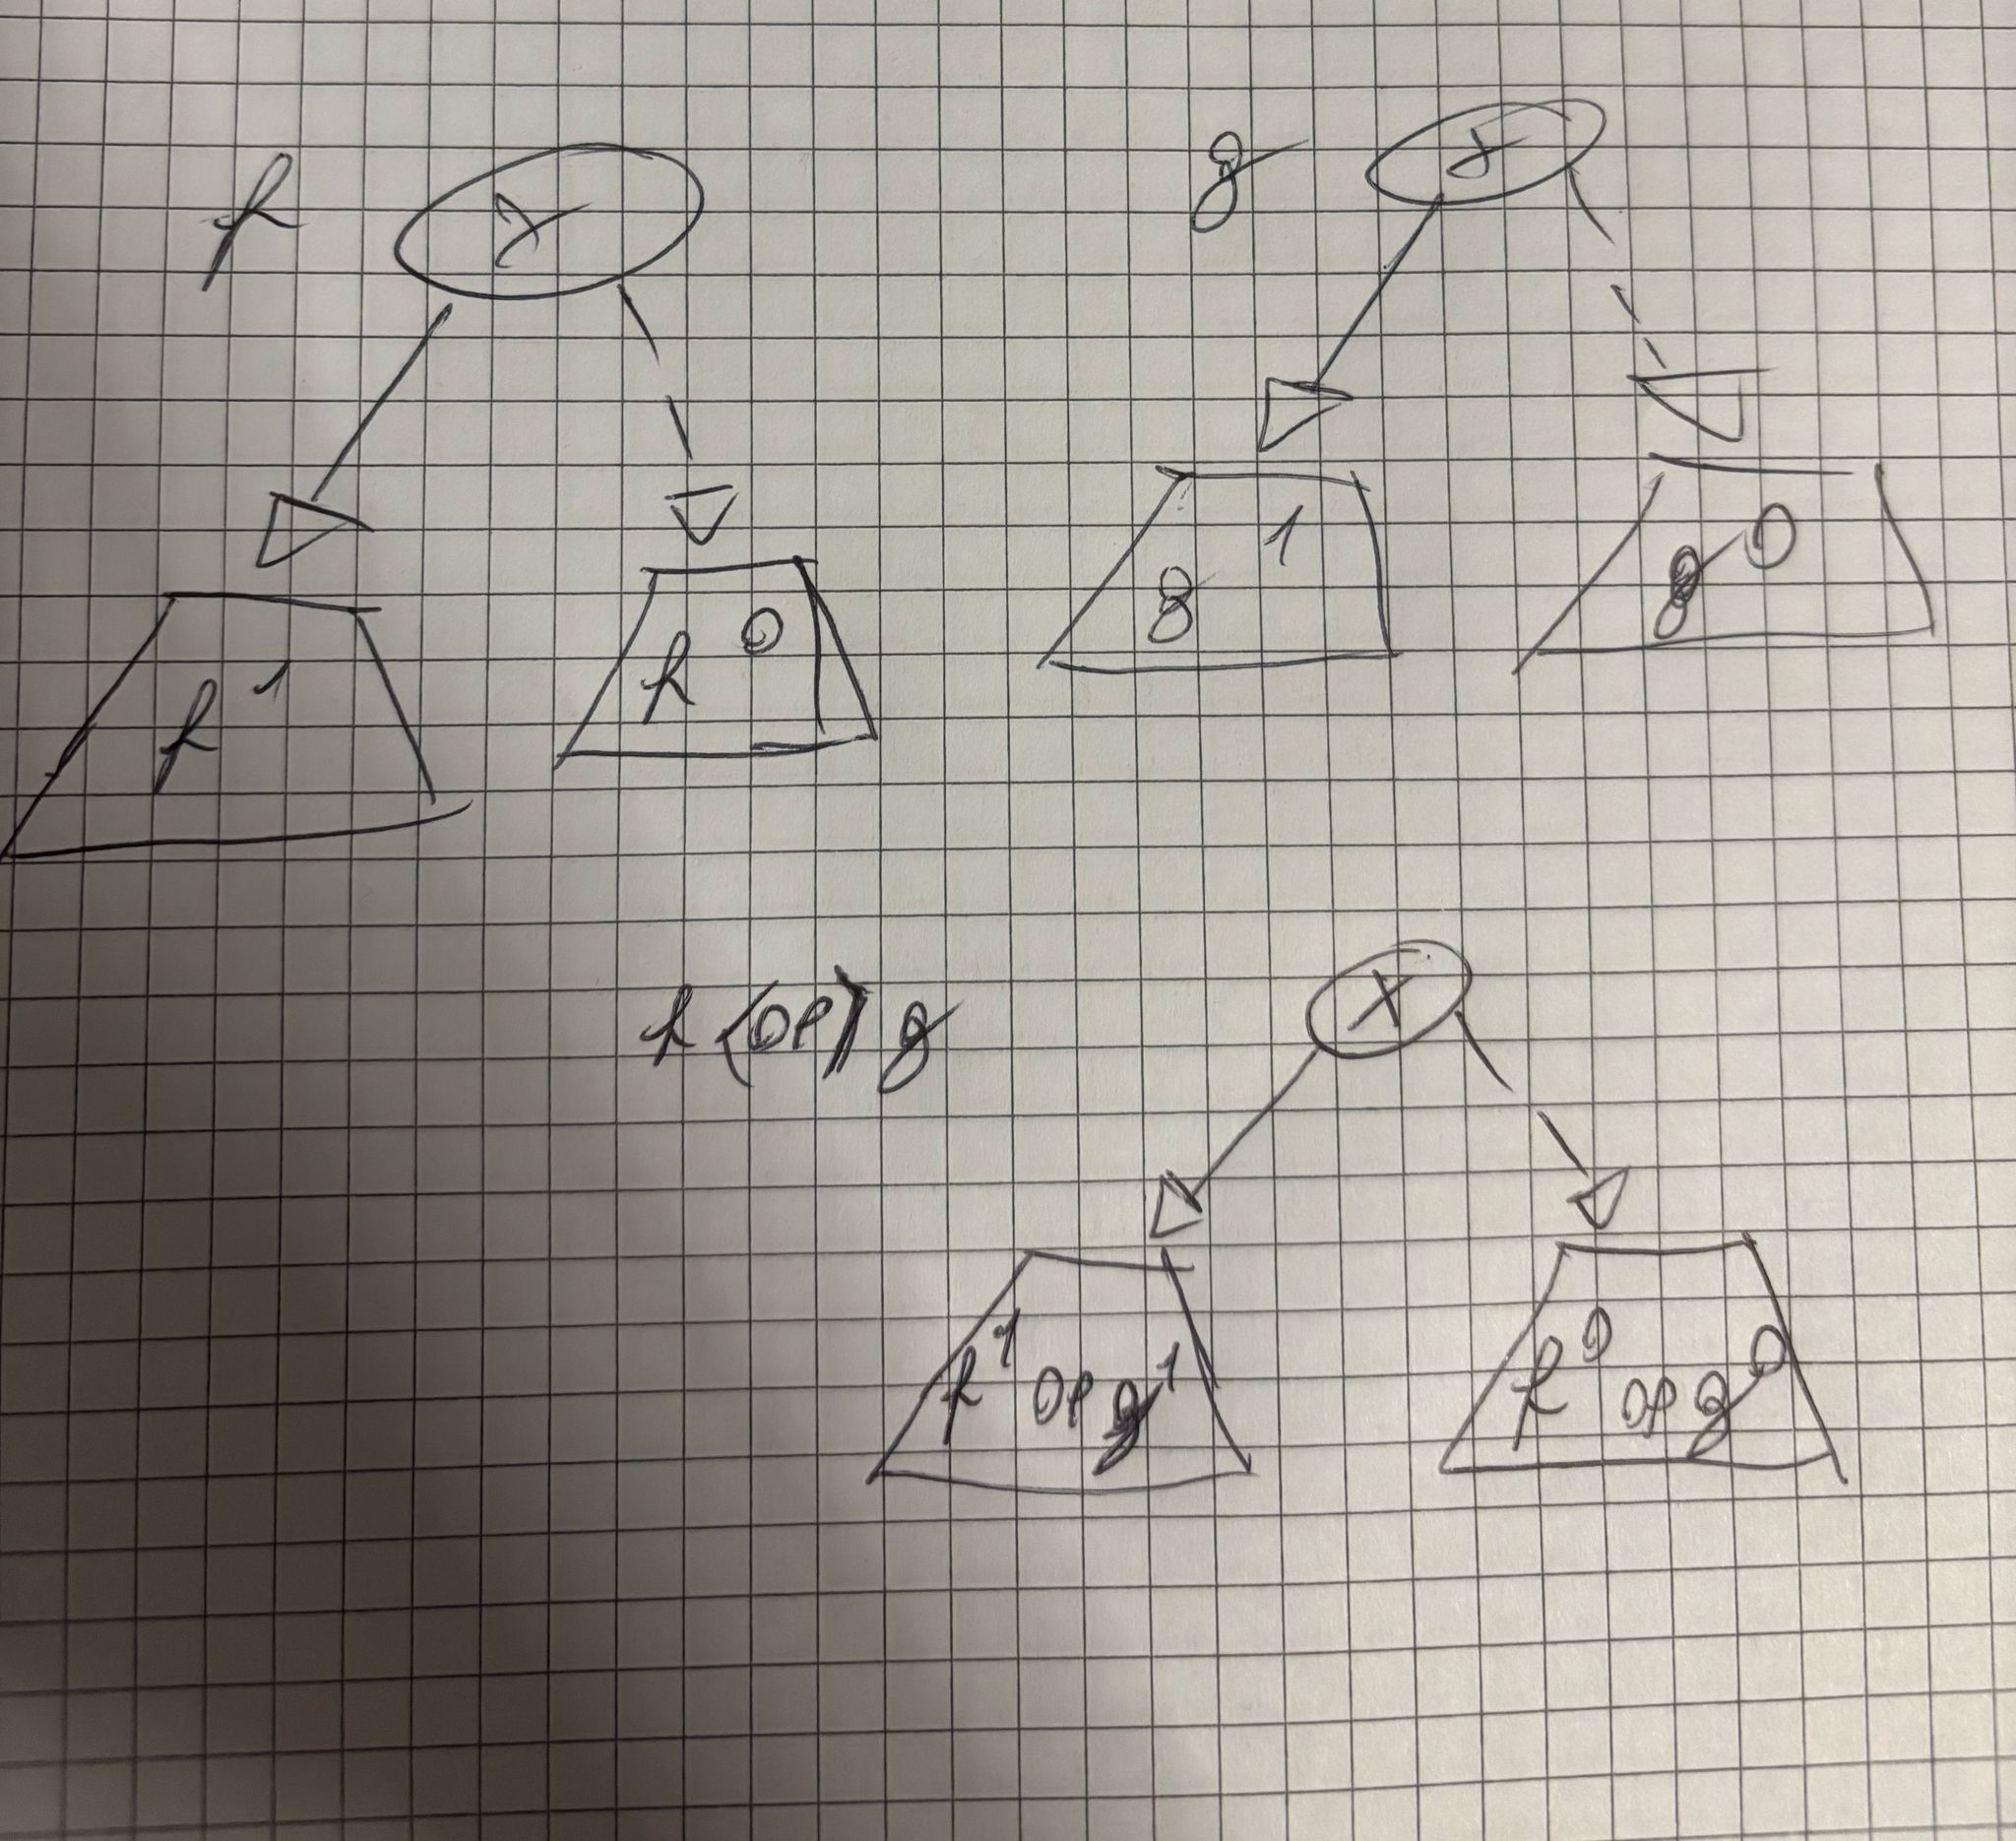
\includegraphics[max width=\linewidth, max height=0.38\textheight, keepaspectratio]{Resources/applySameLabel.jpg}
    \caption{apply con stessa variabile}
    \label{fig:apply1}
\end{figure}

quindi possiamo scrivere $f \langle op \rangle g = \bar{x} \cdot (f^0 \langle op \rangle g^0) + x \cdot (f^1 \langle op \rangle g^1)$  procedere ricorsivamente sulle funzioni $(f^0 \langle op \rangle g^0)$ e $(f^1 \langle op \rangle g^1)$. Intuitivamente è come se il + nell'espansione di shannon della funzione $f \langle op \rangle g$ fosse il nodo decisionale del nuovo obdd.

Se invece le due radici hanno variabili diverse si suppone che una delle due venga prima dell'altra nell'ordine, ad esempio assumiamo che $x$ venga prima di $y$.
\vspace{-10pt}
\begin{figure}[H]
    \centering
    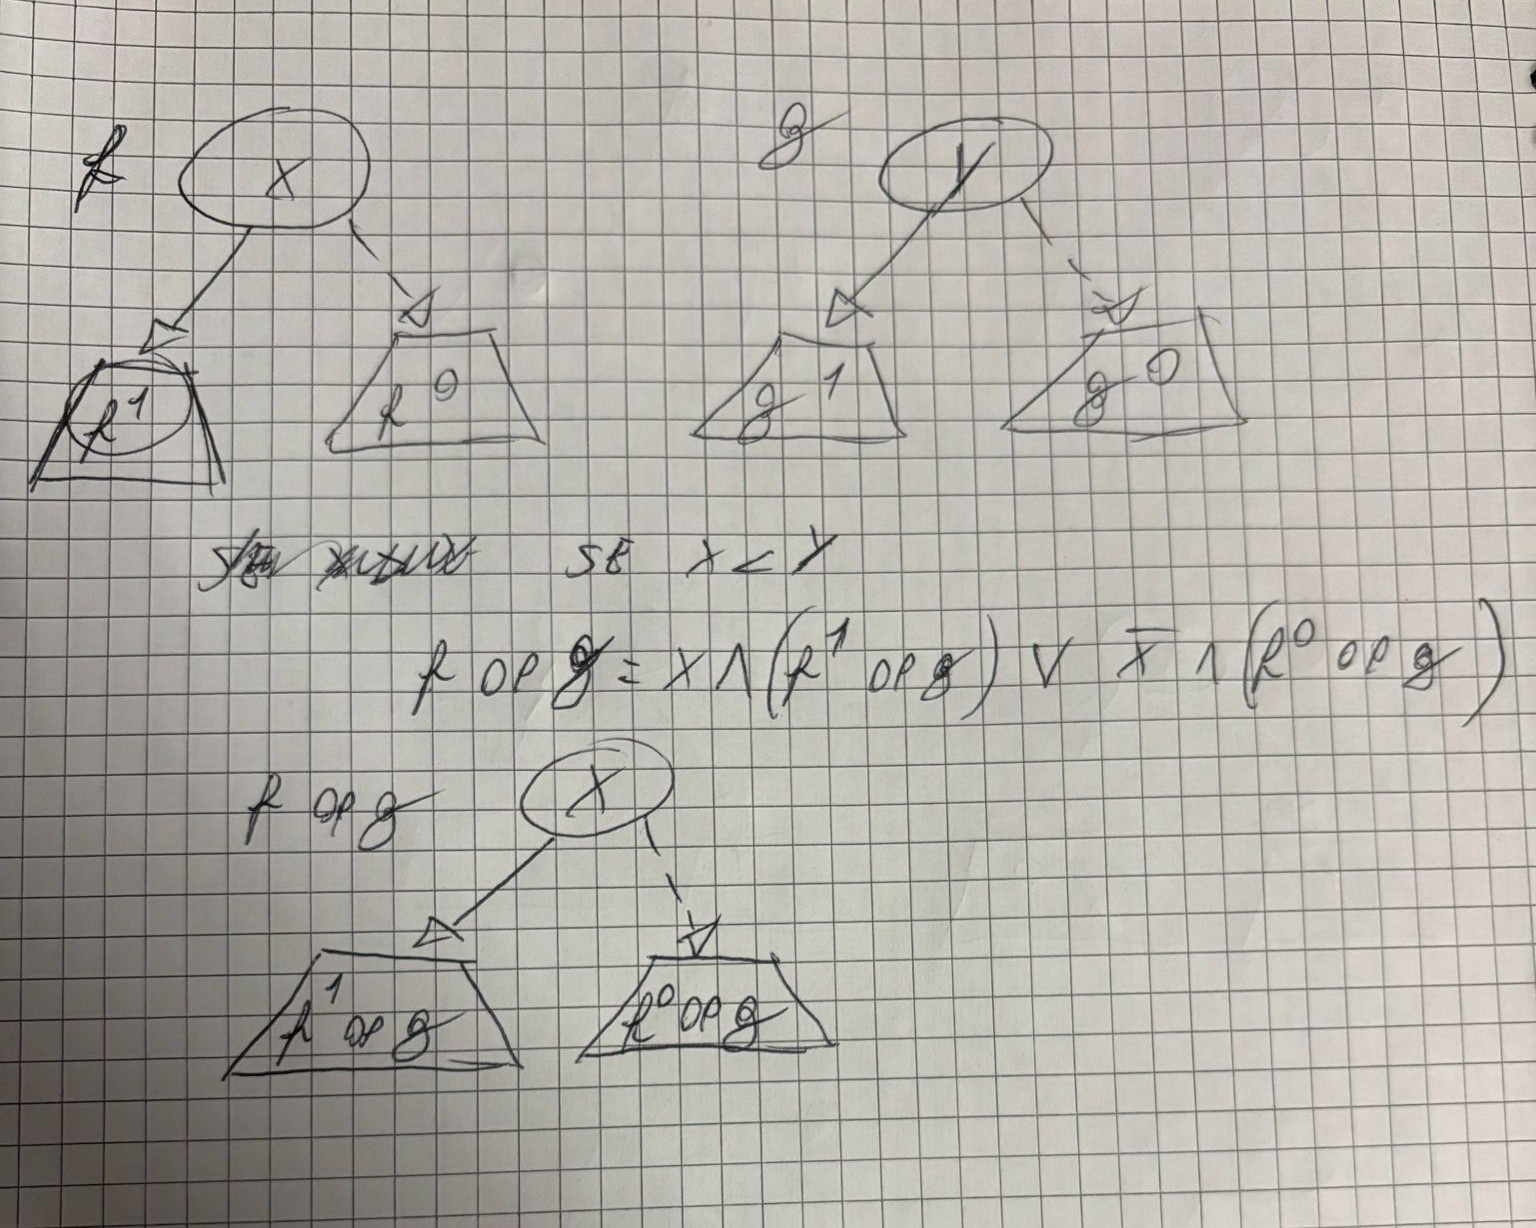
\includegraphics[max width=\linewidth, max height=0.35\textheight, keepaspectratio]{Resources/applyNoSameLabel.jpg}
    \caption{apply con variabili diverse}
    \label{fig:apply2}
\end{figure}

anche in questo caso si procede ricorsivamente sulle funzioni $(f^0 \langle op \rangle g)$ e $(f^1 \langle op \rangle g)$

\end{document}